%----------------------------------------------------------------
%
%  File    :  thesis.tex
%
%  Authors :  Keith Andrews, IICM, TU Graz, Austria
%             Manuel Koschuch, FH Campus Wien, Austria
%			  Sebastian Ukleja, FH Campus Wien, Austria
% 
%  Created :  22 Feb 96
% 
%  Changed :  14 Oct 2020
%
%  For suggestions and remarks write to: sebastian.ukleja@fh-campuswien.ac.at
% 
%----------------------------------------------------------------

% --- Setup for the document ------------------------------------

%Class for a book like style:
\documentclass[11pt,a4paper,oneside]{scrbook}
%For a more paper like style use this class instead:
%\documentclass[11pt,a4paper,oneside]{thesis}

%input encoding for windows in utf-8 needed for Ä,Ö,Ü etc..:
\usepackage[utf8]{inputenc}
%input encoding for linux:
%\usepackage[latin1]{inputenc}
%input encoding for mac:
%\usepackage[applemac]{inputenc}

\usepackage[english]{babel}
% for german use this line instead:
%\usepackage[ngerman]{babel}

%needed for font encoding
\usepackage[T1]{fontenc}

% want Arial? uncomment next two lines...
%\usepackage{uarial}
%\renewcommand{\familydefault}{\sfdefault}

%some formatting packages
\usepackage[bf,sf]{subfigure}
\renewcommand{\subfigtopskip}{0mm}
\renewcommand{\subfigcapmargin}{0mm}

%For better font resolution in pdf files
\usepackage{lmodern}

\usepackage{url}

%\usepackage{latexsym}

\usepackage{geometry} % define pagesize in more detail


\usepackage{colortbl} % define colored backgrounds for tables

\usepackage{courier} %for listings
\usepackage{listings} % nicer code formatting
\lstset{basicstyle=\ttfamily,breaklines=true}

\usepackage{graphicx}
  \pdfcompresslevel=9
  \pdfpageheight=297mm
  \pdfpagewidth=210mm
  \usepackage[         % hyperref should be last package loaded
    pdftex, 		   % needed for pdf compiling, DO NOT compile with LaTeX
    bookmarks,
    bookmarksnumbered,
    linktocpage,
    pagebackref,
    pdfview={Fit},
    pdfstartview={Fit},
    pdfpagemode=UseOutlines,                 % open bookmarks in Acrobat
  ]{hyperref}
\DeclareGraphicsExtensions{.pdf,.jpg,.png}
\usepackage{bookmark}

\usepackage[title]{appendix}

%paper format
\geometry{a4paper,left=30mm,right=25mm, top=30mm, bottom=30mm}

% --- Settings for header and footer ---------------------------------
\usepackage{scrlayer-scrpage}
\clearscrheadfoot
\pagestyle{scrheadings}
\automark{chapter}

%Left header shows chapter and chapter name, will not display on first chapter page use \ihead*{\leftmark} to show on every page
\ihead{\leftmark} 	
%\ohead*{\rightmark}	%optional right header
\ifoot*{Student}		%left footer shows student name
\ofoot*{\thepage}		%right footer shows pagination
%---------------------------------------------------------------------

%Start of your document beginning with title page
\begin{document}


% --- Main Title Page ------------------------------------------------
\begin{titlepage}
\frontmatter

\begin{picture}(50,50)
\put(-70,40){\hbox{
\includegraphics{images/logo.png}}}
\end{picture}

\vspace*{-5.8cm}

\begin{center}

\vspace{6.2cm}

\hspace*{-1.0cm} {\LARGE \textbf{Hardening Kubernetes Clusters\\}}
\vspace{0.2cm}
\hspace*{-1.0cm}Reducing Attack Surface in Kubernetes by means of Rootless Containers, Network Policies and Role Based Access Control\\

\vspace{2.0cm}

\hspace*{-1.0cm} { \textbf{Bachelor Thesis\\}}

\vspace{0.65cm}

\hspace*{-1.0cm} Submitted in partial fulfillment of the requirements for the degree of \\

\vspace{0.65cm}

\hspace*{-1.0cm} \textbf{Bachelor of Science in Engineering\\}

\vspace{0.65cm}

\hspace*{-1.0cm} to the University of Applied Sciences FH Campus Wien \\
\vspace{0.2cm}
\hspace*{-1.0cm} Bachelor Degree Program: Computer Science and Digital Communications \\

\vspace{1.6cm}

\hspace*{-1.0cm} \textbf{Author:} \\
\vspace{0.2cm}
\hspace*{-1.0cm} Guntram Björn Klaus \\

\vspace{0.7cm}

\hspace*{-1.0cm} \textbf{Student identification number:}\\
\vspace{0.2cm}
\hspace*{-1.0cm} c2110475170 \\

\vspace{0.7cm}

\hspace*{-1.0cm} \textbf{Supervisor:} \\
\vspace{0.2cm}
\hspace*{-1.0cm} BSc. MSc. Bernhard Taufner \\

\vspace{0.7cm}

% Reviewer if needed
%\hspace*{-1.0cm} \textbf{Reviewer: (optional)} \\
%\vspace{0.2cm}
%\hspace*{-1.0cm} Title first name surname \\


\vspace{1.0cm}

\hspace*{-1.0cm} \textbf{Date:} \\
\vspace{0.2cm}
\hspace*{-1.0cm} dd.mm.yyyy \\

\end{center}
\end{titlepage}

\newpage

\vspace*{16cm}
\setcounter{page}{1}

% --- Declaration of authorship ------------------------------------------
\hspace*{-0.7cm} \underline{Declaration of authorship:}\\\\
I declare that this Bachelor Thesis has been written by myself. I have not used any other than the listed sources, nor have I received any unauthorized help.\\\\
I hereby certify that I have not submitted this Bachelor Thesis in any form (to a reviewer for assessment) either in Austria or abroad.\\\\
Furthermore, I assure that the (printed and electronic) copies I have submitted are identical.
\\\\\\
Date: \hspace{6cm} Signature:\\

% --- English Abstract ----------------------------------------------------
\cleardoublepage
\chapter*{Abstract}
(E.g. ``This thesis investigates...'')

% --- German Abstract ----------------------------------------------------
\cleardoublepage
\chapter*{Kurzfassung}
(Z.B. ``Diese Arbeit untersucht...'')


% --- Abbrevations ----------------------------------------------------
\chapter*{List of Abbreviations}
\vspace{0.65cm}

\begin{table*}[htbp]
		\begin{tabular}{ll}
			ARP & Address Resolution Protocol \\
			GPRS & General Packet Radio Service \\
			GSM  &  Global System for Mobile communication \\
			WLAN & Wireless Local Area Network \\
		\end{tabular}
\end{table*}

% --- Key terms ----------------------------------------------------
\newpage
\chapter*{Key Terms}
\vspace{0.65cm}

\begin{itemize}
	\setlength{\itemsep}{0pt}
	\item[] GSM
	\item[] Mobilfunk
	\item[] Zugriffsverfahren
\end{itemize}

% --- Table of contents autogenerated ------------------------------------
\newpage
\tableofcontents
\thispagestyle{empty}

% --- Begin of Thesis ----------------------------------------------------
\mainmatter
\chapter{Introduction}
\label{chap:intro}

\newpage
\section{Background: Enterprises and Cloud}
\label{sec:Unterkapitel1}

\section{Research Objectives}
\label{sec:Unterkapitel2}

\newpage
\section{Methodology}
\label{sec:Unterkapitel3}


\section{Structure}
\label{sec:Unterkapitel4}

\newpage
\chapter{Concepts}
\label{chap:back}


\section{Containervirtualization}
\label{sec:Unterkapitel21}

\newpage
\subsection{Linux Kernel}
\newpage
\subsection{Container Images}
\newpage
\subsection{Container Runtimes}

\newpage
\section{Kubernetes}
\label{sec:Unterkapitel23}

\subsection{Components}
\newpage
\newpage
\subsection{Cluster Architecture}
\newpage
\subsection{Cluster Objects}
\newpage
\newpage
\chapter{Literature Review}
Kubernetes is highly customizable and offers a range of configuration options which determine the security posture of
individual applications and the cluster as a whole. 
The purpose of this literature review is to explore the security threat landscape of Kubernetes environments. 
Specifically, recurring concepts and common denominators across vulnerabilities shall be identified and discussed. For this, 
the database of Common Vulnerabilities and Exposures (CVE), the IEEE database, the ACM digital library and the official
Kubernetes feed of CVEs are queried using keywords pertaining to Container and Kubernetes Security. In order to minimize manual 
labor to research the sheer amount of CVE reports, a Python script was developed to automate the research. The acquired papers, 
articles and CVE descriptions are skimmed through. The most relevant results are narrowed down and selected for closer inspection. 
It shall be noted that Kubernetes vulnerabilities do not only entail standard Kubernetes components, but also add-ons deployed on
top of 'plain' Kubernetes. Such can be the Nginx Ingress-Controller, a Service-Mesh, CI/CD tools closely embedded into Kubernetes
and more. Generally, this can be anything that extends the Kubernetes API through Custom Resource Definitions (CRDs).    
\\
CVE:
The main goal of the Common Vulnerabilities and Exposures (CVE) Programme is to identify vulnerabilities in a unique way and link particular 
code bases (such as common libraries and software) to those vulnerabilities. The usage of CVEs guarantees that when discussing or exchanging 
information about a specific vulnerability, two or more parties can confidently refer to a CVE identifier (CVE numbers). The CVE program 
defines a vulnerability as: 
\\
"A weakness in the computational logic (e.g., code) found in software and hardware components that, when exploited, results in a negative impact 
to confidentiality, integrity, or availability. Mitigation of the vulnerabilities in this context typically involves coding changes, but could 
also include specification changes or even specification deprecations (e.g., removal of affected protocols or functionality in their entirety)."
\\
In addition, the Common Vulnerability Scoring System (CVSS) "is a method used to supply a qualitative measure of severity"CITE HERE. 
The three metric groups that make up CVSS are Base, Temporal, and Environmental. Once the Temporal and Environmental metrics have been scored, 
the Base metrics produce a score between 0 and 10. A vector string, which is a condensed textual representation of the values required to calculate 
the score, is another way to visualise a CVSS score. Therefore, enterprises, organisations, and governments that require precise and consistent 
vulnerability severity scores can benefit greatly from using CVSS as a standard measurement system. CVSS is frequently used to prioritise vulnerability 
mitigation efforts and to determine the severity of vulnerabilities found on a system. All publicly available CVE records are assessed by the National
Vulnerability Database (NVD).
\\
There are multiple public APIs which allow for querying for various information on CVEs. The goal of the Python script is to quickly
collect CVEs for a given keyword with a CVSS base score higher than a given integer. To achieve this, the OpenCVE project's API is queried for all CVEs
containing a given keyword. The returned JSON response is filtered for the CVE number. This number is then used to call the NVD API of the NIST organization,
whose response can then be filtered for the base severity score according to the CVSS framework. As a result, interesting insights can be gained by
programmatic means. The following figure depicts the collected data on CVE's for the keyword 'Kubernetes'.
\\
\\
Total results: 269
\\
Base score average: 7.13
\\
Base score median: 7.2
\\
Base score modus: 6.5
\\
\\

\begin{figure}[htbp]
	  \centering
		    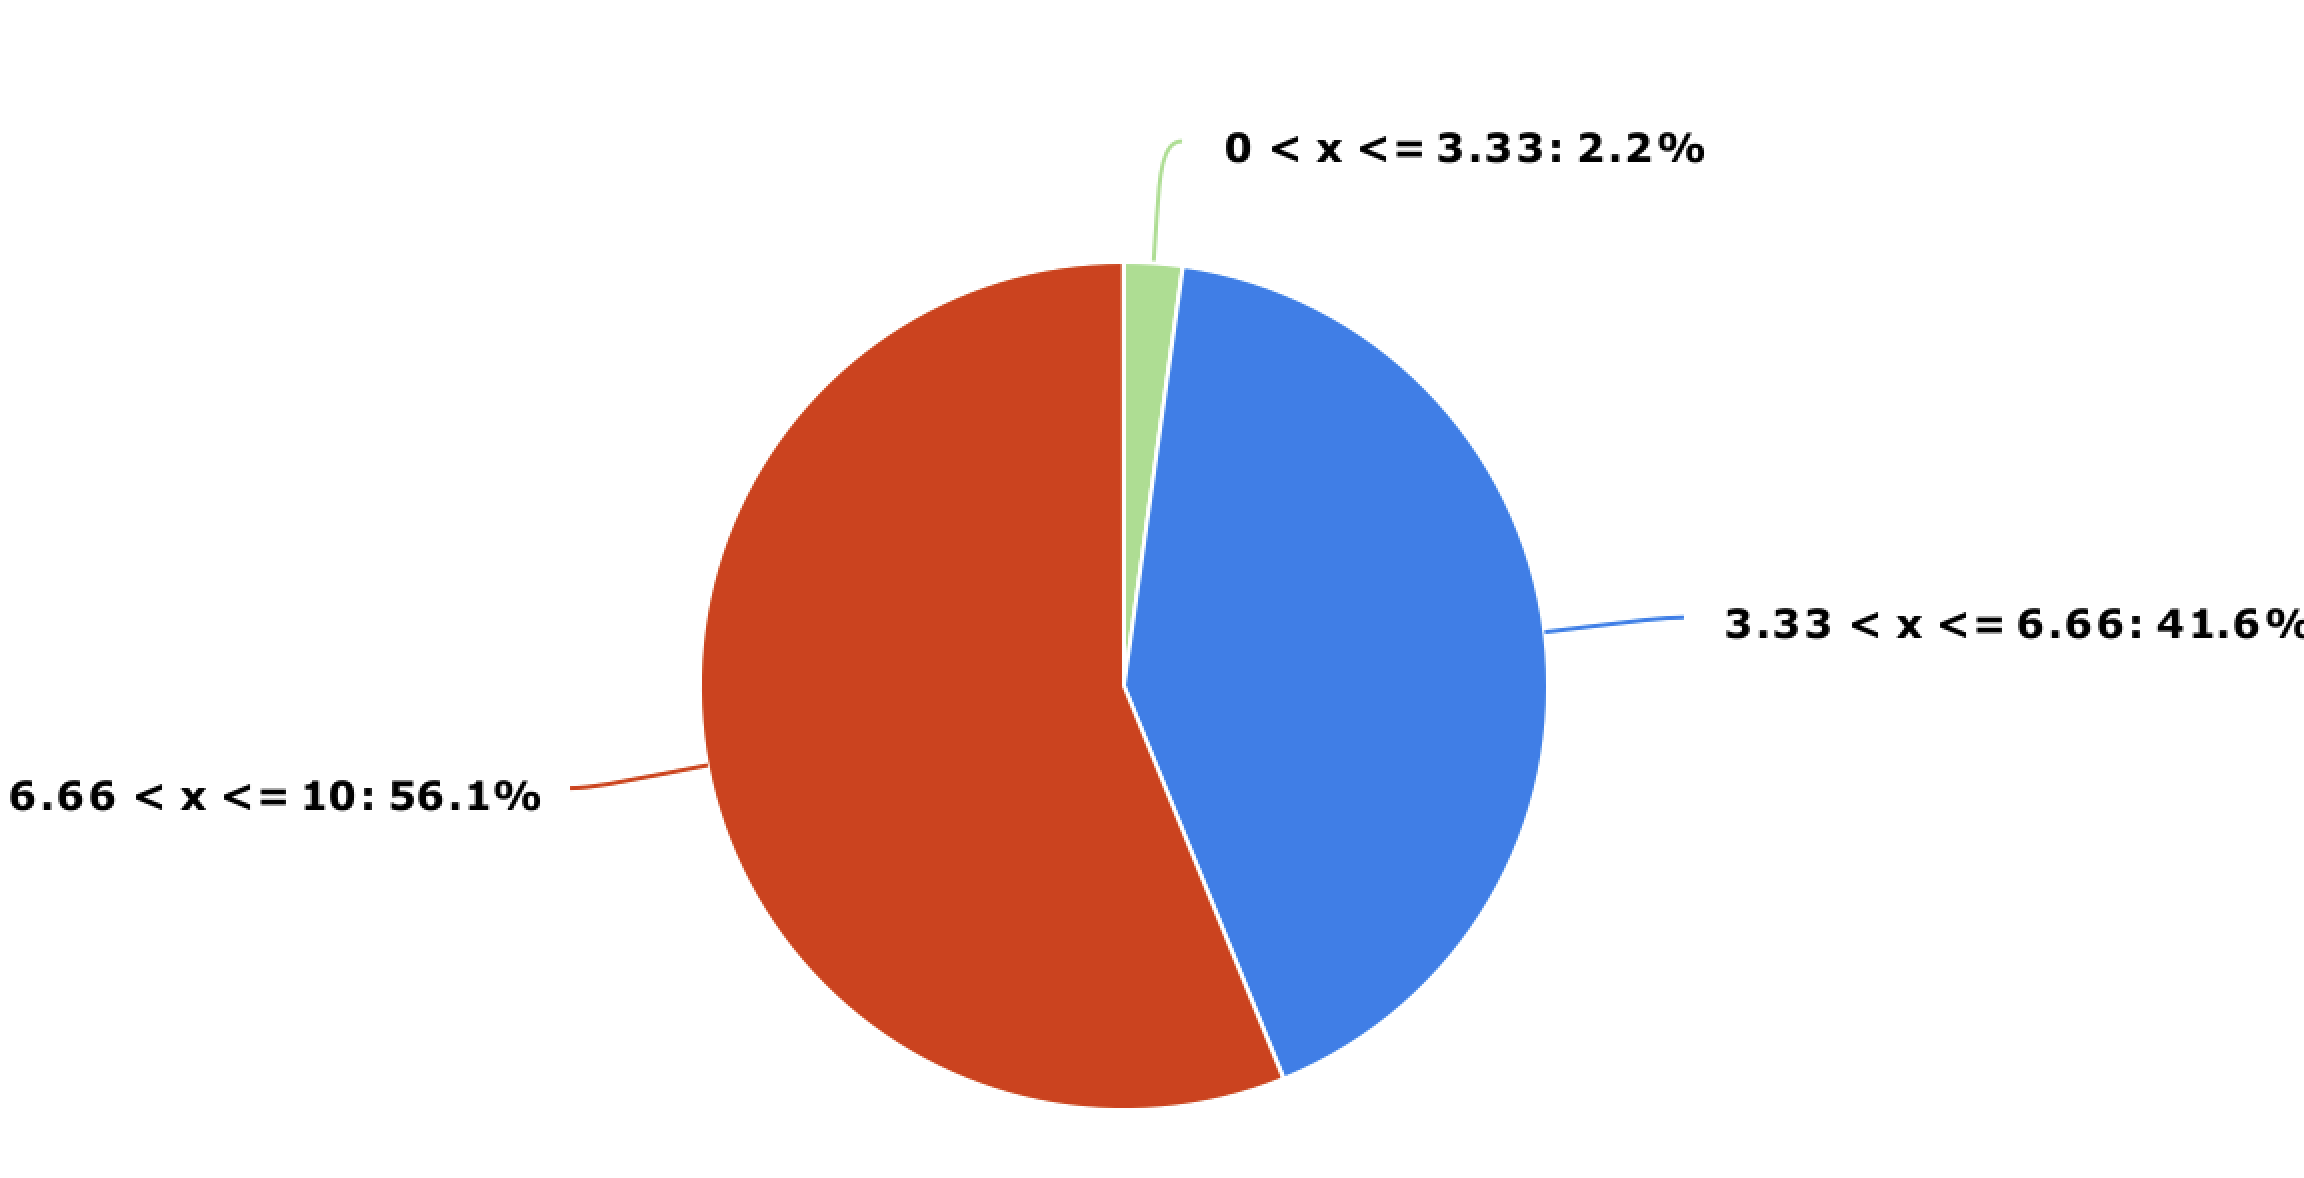
\includegraphics[height=5cm]{../images/cvepie}
	  \caption{Makeup of base scores of CVEs about Kubernetes}
	  \label{fig:cvepie}
\end{figure}


The chart below depicts the collected data on CVE's containing either of the keywords 'containerd', 'CRI-O' or 'Docker Container'.
\\
\\
Total results: 75
\\
Base score average: 7.9
\\
Base score median: 7.8
\\
Base score modus: 9.8
\\
\\
\begin{figure}[htbp]
  \centering
      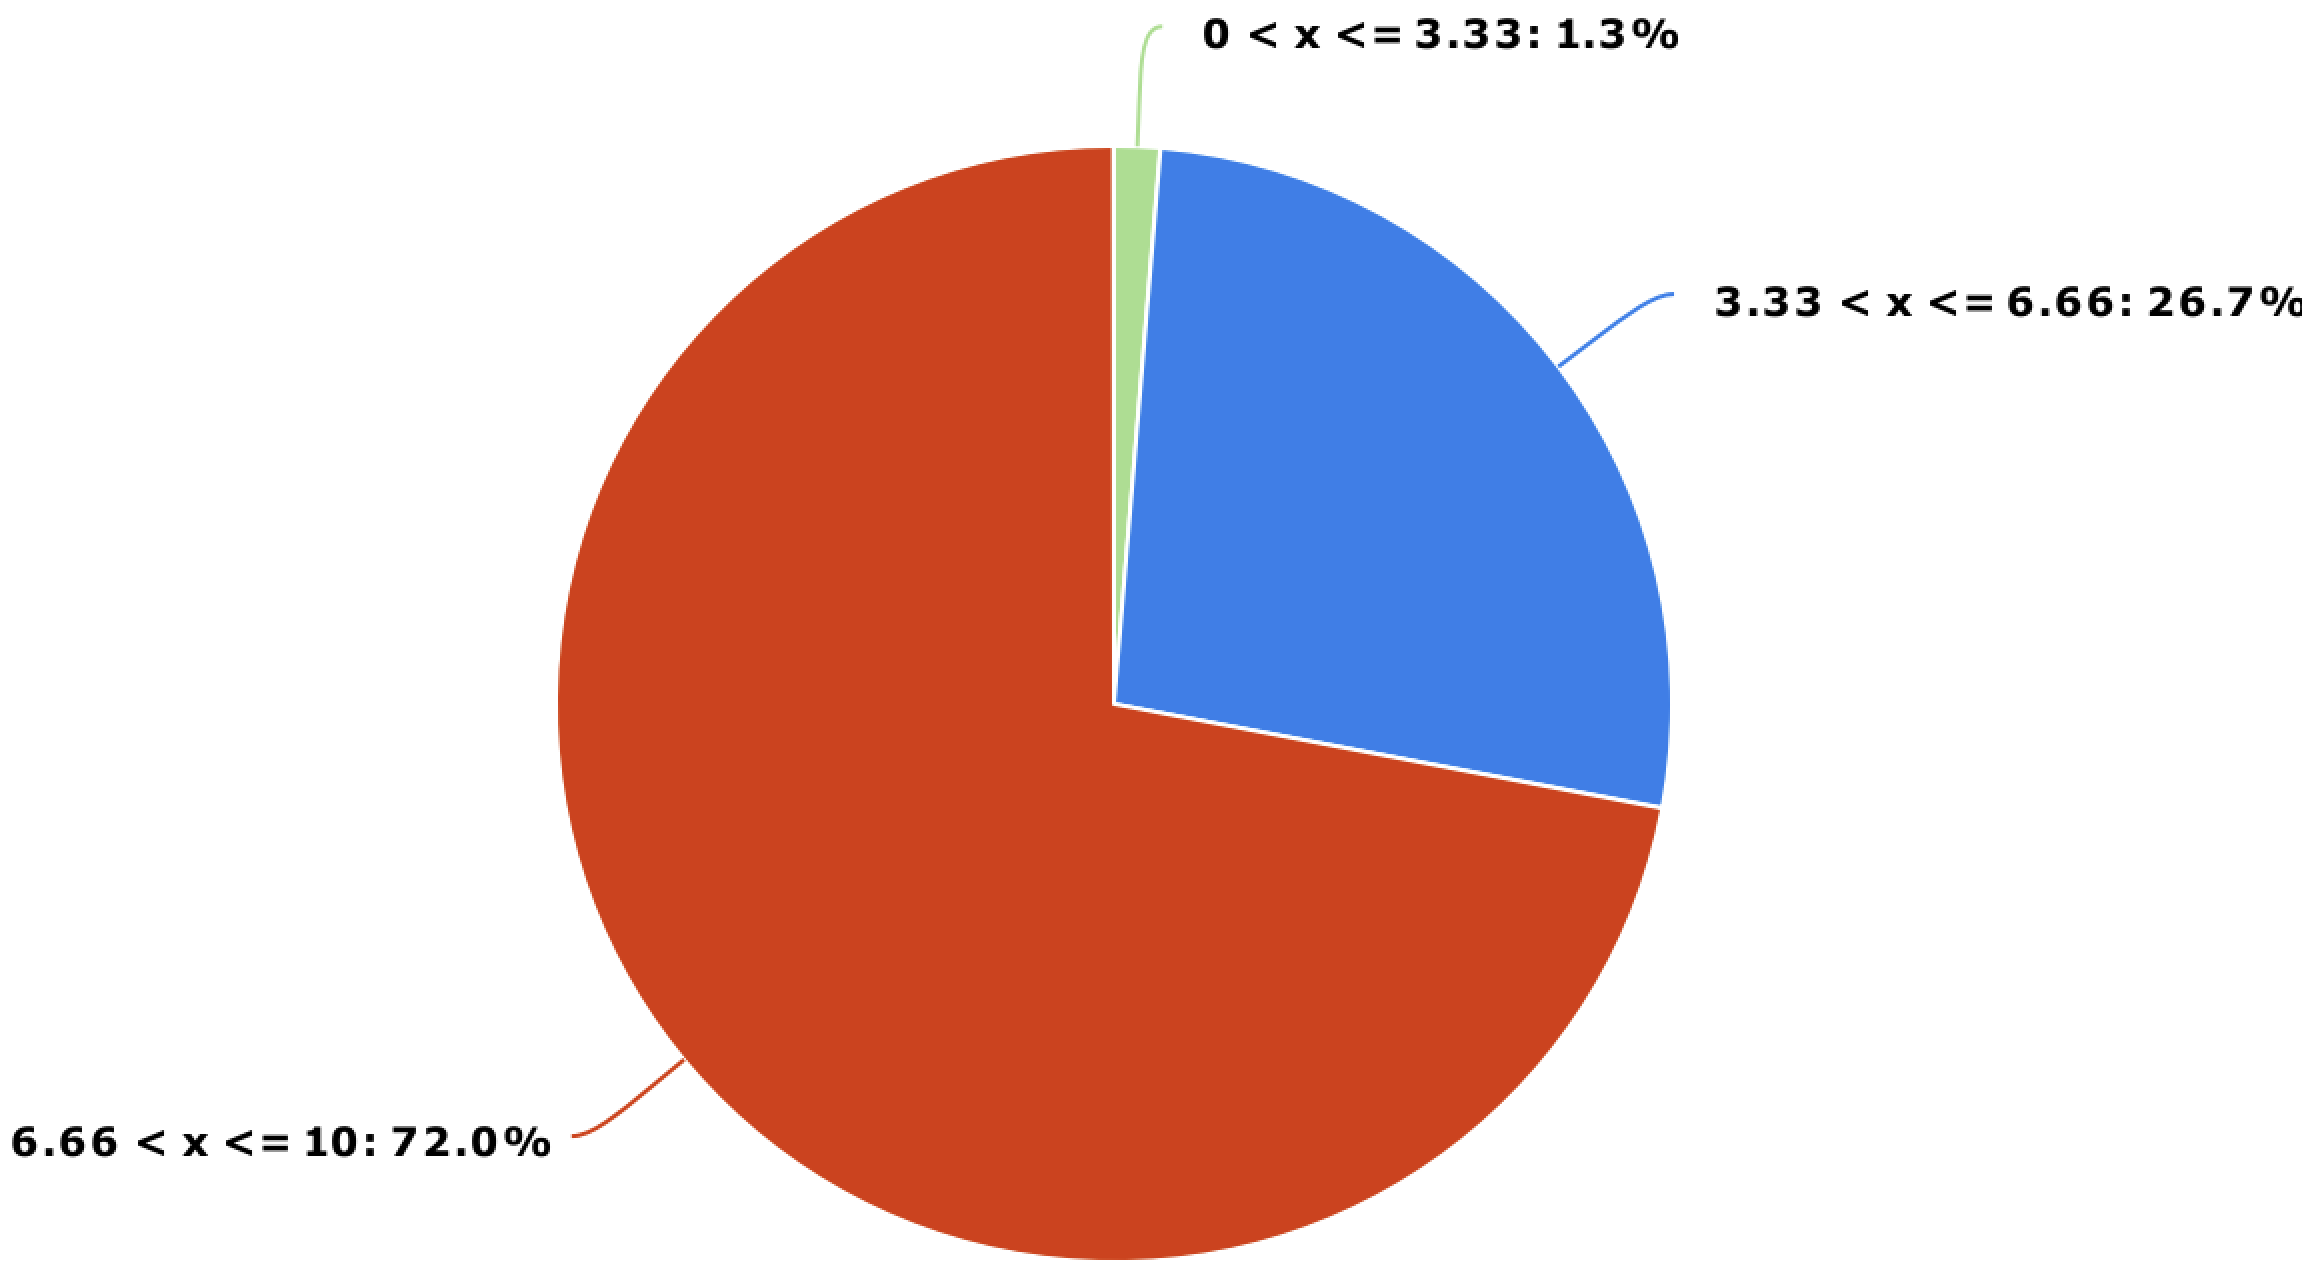
\includegraphics[height=5cm]{../images/cvepie2}
  \caption{Makeup of base scores of CVEs about Kubernetes}
  \label{fig:cvepie}
\end{figure}

Based on collected data, it is noticeable that CVSS base severity scores in the realm of Containervirtualization and Kubernetes tend toward extremes
on the higher end. For the keyword 'Kubernetes', more than half of CVEs are rated with a base score higher than 6.66, while there are hardly any 
scores smaller than 3.33. For CVEs that draw on popular container runtimes, an overwhelming majority close to 75 percent of cases holds base scores 
between 6.66 and 10. Here, once again, scores smaller than 3.33 are low. These two observations additionally emphasize the necessity for clear 
security measures when orchestrating containers in Kubernetes. 
The script enables to quickly retrieve the tendencially more severe vulnerabilities. Some CVEs marked with a CVSS base scores higher than 7 shall
be explored in the following chapters.
\\
\\
It is evident that the reliance on Kubernetes comes with the need of a clear security initiative. According to RedHat's report on 
the state of Kubernetes security of 2022, more than ninety percent of polled organizations underwent at least one security incident
in their Kubernetes environment, which, in a third of cases, lead to the loss of revenue or customers. The majority of these incidents 
were detections of misconfigurations. About a third of respondents reported major vulnerabilities and runtime security incidents 
in relation to containers and/or Kubernetes which required immediate remediation. In a more recent, similar report conducted by RedHat in
2023, two thirds of respondents had to delay or slow down application deployments because of security concerns. This is a significant
increase compared to the 2022 survey, where just over half of participants experienced delays. Three of the most frequently mentioned 
advantages of containerization include quicker release cycles, quicker bug fixes, and increased flexibility to operate and manage applications. 
But if security is neglected, you can lose out on containerization's biggest benefit: agility.
It becomes apparent that Kubernetes is not something that is installed once and then never looked at again. Rather, a container-based 
environement that leverages this orchestration technology requires attention for detail and constant, rigurous inspection, despite the 
great amount of abstraction provided and due to its highly customizable nature.  CITE REDHAT 2022 2023
\\
Container Escape
\\
Major vulnerabilities include those which fall under the category of a so called container-escape. Since a container is intended to be a 
runtime environment isolated from the underlying host, the concept of a container-escape relates to performing an exploit that breaks the confines 
of exactly this isolation, resulting in full or limited access to the underlying host machine and/or network. A study conducted by Reeves 
et al. at the end of 2021 investigates the susceptibility of different container runtime systems to escape-exploits by studying a batch of CVE 
reports. The study identifies three main causes for container escapes. 
First, mishandled file descriptors, if for example left accessible from within a container under /proc directory, provides malicious actors read and write 
access to the underlying host filesystem, as seen in CVE-2019-5736. In this reported vulnerability, a container is set up with a symlink from the 
container's entrypoint to proc/self/exe, which points back to its runC binary, which instantiated the container process. In addition, the container 
carries a harmful file which is designed to overwrite the  file descriptors of any excecuting process that loads it. If an unknowing person executes 
a binary within the container, which has been manipulated to symlink to /proc/self/exe, the harmful file is able to overwrite the runC binary. 
The next time another, unrelated container is spawned, it is done by the compromised runC binary. 
Secondly, missing access control to runtime components could enable adversaries to gain access to UNIX sockets on the host, as reported in 
CVE-2020-15257. Here, it was possible to connect to the containerd socket, thus enabling actors to issue API commands to freely create new containers
on the host, unconstrained by Apparmor, seccomp, or Linux capabilities. 
Thirdly, under 'adversary-controlled host execution' problems of similar fashion to mishandled file descriptors are mentioned. In this case however, 
vulnerability exposure starts with host binaries being executed in the container context, which makes it a target for manipulation. 
In CVE-2019-101(44–47), the shared library "libc.so.6" is altered in such a way that it mounts the host filesystem when loaded. The new shell loads 
"libc.so" when the administrator runs "rkt-enter", which is the /bin/bash command by default, to create a new shell in the container. This sets off malicious 
code embedded in "libc.so", which uses the mknod syscall to construct a block device of the host root filesystem inside the container. 
As a result, the adversary is able to read and write to the host filesystem. 
\\
CVE-2022-0811, which is barely discussed in papers due to its young nature, reports a sophisticated container escape possibility of the CRI-O container engine.
Generally, the interface of the Linux kernel accepts parameters which control its behavior. This interface is consumed by CRI-O to set kernel options for a pod. 
However, the parameter input string is not checked or sanitized, which allows for injecting additional, otherwise undesired parameters. Specifically in the
example of CVE-2022-0811, the "kernel.core\_pattern" kernel parameter is specified within the parameter of the safe "kernel.shm\_rmid\_forced" parameter, 
which controls the kernel's reaction to a core dump. If a core dump is done in a CRI-O container, the parameter states the execution of a malicious binary. 
This binary sits inside the container but is invoked on the host in the root context of the container from the perspective of the kernel.
\\
CVE-2022-23648 is another vulnerability related to container-escape, this time found in Containerd, a popular Kubernetes runtime. This vulnerability lies in 
Containerd's CRI plugin that handles OCI image specs containing "Volumes". An attacker can exploit this vulnerability by adding a Volume containing path traversal 
to the image. This allows them to copy arbitrary files from the host to a container mounted path. More specifically, The vulnerability resides in the 
"copyExistingContents" function in Containerd's code. This function copies the files from the attacker-controlled volume path to a temporary folder that is later 
mounted inside a container. An attacker can trick this function into copying arbitrary files from the host filesystem using path traversal.
This can lead to the disclosure of confidential information. The severity of this vulnerability is rated as high, with a CVSS base score of 7.5.
\\
CVE-2022-1708 is a vulnerability found in Cri-o, a lightweight container runtime for Kubernetes. This vulnerability is related to the allocation of resources 
without any limits or throttling, which can lead to uncontrolled resource consumption. The official CVE description states: "The ExecSync request runs commands 
in a container and logs the output of the command. This output is then read by CRI-O after command execution, and it is read in a manner where the entire file 
corresponding to the output of the command is read in." It is thus possible to exhaust memory or disk space of the node when CRI-O reads an extensive output 
of the command. The vulnerability is rated as high, with a CVSS base score of 7.5 and targets system availability.
\\
Cilium is an eBPF-based solution for network connectivity between workloads in Kubernetes CLusters. CVE-2022-29179 reports yet another subjection to the risk of 
container breakouts.  The CVE number is not directly about a technique to gain access outside the container, it rather addresses a vulnerability in Cilium given a 
successful container escape. It explicitly mentions root containers as a prerequesite. According to this CVE entry, Cilium's service account in versions prior to
version 1.9.16 allowed for escalating privileges to those of a cluster admin. This gave adversaries the ability to delete cluster resources such as Pods and Nodes. 
The entry is marked with a base score of 8.2 which is considered high.
\\
CVE-2020-8554:
In the case of CVE-2020-8554, the source is a design defect in the External IPs and Load Balancer IPs components of Kubernetes Services. An application running on a collection 
of pods can be exposed as a network service in an abstract manner using Kubernetes Services. One or more IPs are used to access a service. When the cluster's nodes 
are deployed, traffic intended for the service IPs will be routed through one of the backing pods that comprise the service. By assigning IP addresses that are already 
being used by other endpoints (internal or external), a malevolent user might intercept all cluster traffic directed towards those IP addresses. 
With the service shown below, it used to be possible to intercept UDP traffic to IP 8.8.8.8, which is Google's DNS server, and direct it to the "evil-dns-server" 
pod when it is deployed to the cluster.

\begin{figure}[htbp]
  \centering
      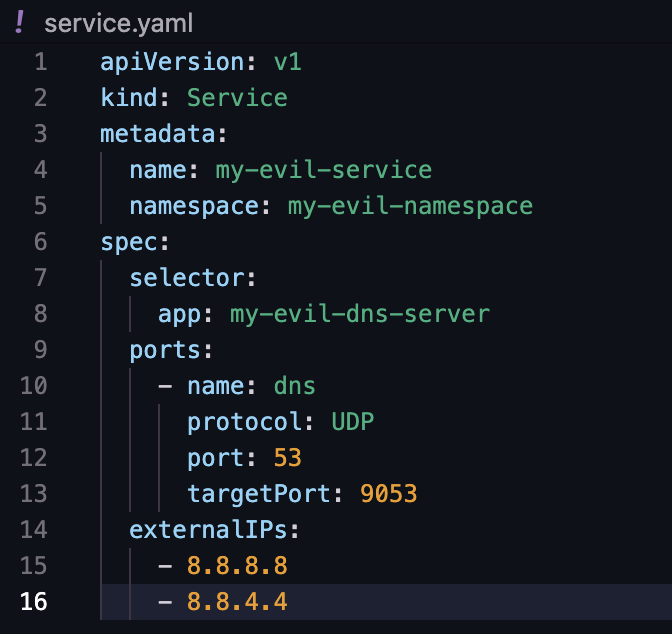
\includegraphics[height=5cm]{../images/service}
  \caption{YAML declaration of a malicious service}
  \label{fig:cvepie}
\end{figure}

Of the more recent vulnerabilities with high severity, CVE-2023-5043 and CVE-2023-5044 report problems with the Nginx Ingress Controller. 
The Nginx Ingress Controller is a popular add-on to Kubernetes with which cluster incoming traffic is managed. Instead of assigning
each Kubernetes Service an IP and port directly on the underlying node, the Nginx container serves as a single point of entry and acts as a reverse proxy to the cluster
workloads. To expose a cluster workload, a Kubernetes resource of type 'Ingress' is defined. Within this YAML definition, the nginx ingress controller picks up custom configuration
through so called annotation snippets. This allows for fine-grained, customized behavior of the controller for a respective service. It was however discovered that 
specific declarations of the "nginx.ingress.kubernetes.io/configuration-snippet" and "nginx.ingress.kubernetes.io/permanent-redirect" annotations of an Ingress Object can be 
used to inject arbitrary commands, making it possible to obtain credentials of the said nginx ingress controller. Utilizing this credential, even more cluster secrets could 
be obtained. Multi-tenant environments are most affected by the issue.  
\\
nginx ingress cve 3 CVE-2023-5044:
\\
disclosed tokens CVE-2023-2878
\\
A successful container-escape arguably poses one of the greatest risk in a Kubernetes environment as it provides a starting point from which all three pillars of 
the CIA triad can be targeted: Confidentiality, Integrity, and Availability. Once an attacker gains access of the host, secrets can be read, binaries can be altered,
network traffic can be inspected and resources can be deleted. In contrast, other vulnerabilities 'only' allow for more restricted exploitability. For example, 
CVE-2022-1708, CVE------- and CVE---------- target the availability of the system, but not the confidentiality or integrity of data. The average CVE scores of
\\
The foundation of such attacks is being able to either freely instantiate containers or freely move and operate from inside a container
The most notable ones, which have a severity score above 8, according to the Common Vulnerability 
\\
We see that vulnerabilities vary tremendously in their appearance. CVE so and so targets a tool, CVE so and so targets the actual underlying
kernel of a k8s node. However, all these things can be prevented or alleviated by applying the concept of least privilege to containers, 
access to Kubernetes and the Kubernetes network. For example, if a malicious actor cannot freely create files in any desired directory of a 
compromised container, it significantly reduces his ability to exploit a given vulnerability. Not being able to create that file in the first 
place, due to missing write permissions, would be a major obstacle for performing a container escape. It is not always possible to completely 
avoid a vulnerability. This is due to software bugs and unidentified weaknesses in the code that have passed through the testing and review process. 
\section{State of the Art}
\newpage
\section{CVE Numbers}
\newpage
\section{Incident Reports}
\newpage

\newpage
\chapter{Hardening Measures}
\section{Securing Containers}
\subsection{Linux File Permissions}
\newpage
\subsection{Root versus Rootless}
\newpage
\subsection{Rootless Policy Enforcement}
\newpage
\section{Securing the Network}

Default pod-to-pod network settings, as an example, allow open communication to quickly get a cluster up and running, at the expense of 
security hardening. Network segmentation.....
\subsection{Network Policies}
\newpage
\subsection{Service Mesh}
\newpage
\section{Authentication and Authorization}
\subsection{Role Based Access Control}
\newpage
\subsection{Kubeconfig Keys and Certificates}
\newpage
\subsection{Service Accounts}

\newpage
\chapter{Discussion}
\section{Implications for businesses}
\newpage
\section{Tradeoffs and Difficulties}
\section{Complexity}

\newpage
\chapter{Conclusion}

\newpage
\chapter{Outlook / Future work}

\newpage

% --- Bibliography ------------------------------------------------------

%IEEE Citation [1]
\bibliographystyle{IEEEtran}
%for alphanumeric citation eg.: [ABC19]
%\bibliographystyle{alpha}

% List references I definitely want in the bibliography,
% regardless of whether or not I cite them in the thesis.

\newpage
\addcontentsline{toc}{chapter}{Bibliography}
\bibliography{testBib}

\newpage

% --- List of Figures ----------------------------------------------------

\addcontentsline{toc}{chapter}{List of Figures}
\listoffigures


% --- List of Tables -----------------------------------------------------

\newpage
\addcontentsline{toc}{chapter}{List of Tables}
\listoftables

% --- Appendix A -----------------------------------------------------

\backmatter
\appendix
\begin{appendices}
\chapter{Appendix}

(Hier können Schaltpläne, Programme usw. eingefügt werden.)

\clearpage
\end{appendices}

\end{document}
